\chapter{Konzept und Systemdesign}
\printmyminitoc{1}

\section{Aufbau Schiffsysteme}
Ein Schiff besteht aus vielen verschiedenen Systemen, welche verschiedene Aufgaben haben. In diesem Fall wird das
Steuerungssystem des Schiffes betrachtet. Dabei werden die wichtigen Systeme für die Arbeit abstrahiert, um die
Funktionsweise des Systems zu verstehen.
\begin{figure}[H]
    \centering
    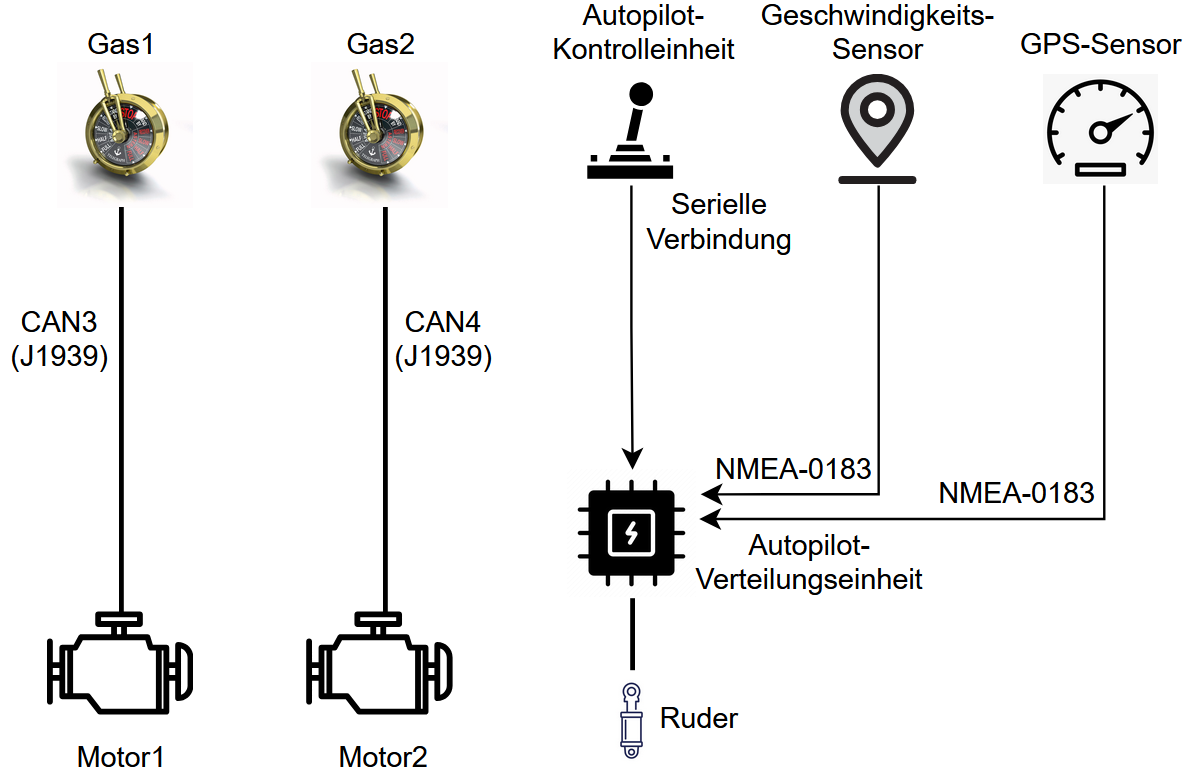
\includegraphics[scale=0.3]{images/limandaSystem.png}
    \caption{Vereinfachte Darstellung der Systeme auf der Limanda}
\end{figure}
Die wichtigen Systeme für diese Arbeit begrenzen sich auf die Gashebel und den Autopiloten. Die beiden Gashebel sind jeweils
mit einem CAN-Bus verbunden. An diesen Bussen werden die Steuerbefehle für die Motoren gesendet. Dort sind unter anderem 
auch Bildschirme für den Schiffsführer angeschlossen. Als Higher-Layer-Protokoll wird J1939 genutzt. \\
Der Autopilot ist ein eigenständiges System, welches über eine serielle Schnittstelle mit dem Ruder verbunden ist.
Dieser hat keine Verbindung zu den Gashebeln oder Motoren. Er kann lediglich Signale an die Rudersteuerung senden.
Dabei ist dieser mit einer seriellen Verbindung an die Rudersteuerung angeschlossen. Diese Verbindung ist unverschlüsselt.
Die Rudersteuerung ist mit dem Ruderstellmotor über eine unbekannte Verbindung angeschlossen. Diese Verbindung ist
jedoch nicht relevant für diese Arbeit.\\



\section{Steuerungslogik des Controllers}
Der benutzte Controller ist ein Xbox Series X Controller. Dieser wurde gewählt, da er eine gute Haptik hat und weit
verbreitet ist. Zusätzlich ist er kabellos und kann somit frei bewegt werden. Um die Steuerung des Schiffes zu
ermöglichen, müssen die Eingaben des Controllers in Steuerbefehle umgewandelt werden. Dies passiert auf dem 
Raspberry Pi. Der Controller wird über Bluetooth mit dem Raspberry Pi verbunden. Dort werden die Eingaben des Controllers
ausgelesen und in einem Python-Programm in Steuerbefehle umgewandelt. \\
Um eine einfache Steuerung zu ermöglichen, wird im folgenden die Tastenbelegung aufgeschlüsselt.
Um alle gewünschten Funktionen umzusetzen, werden nicht alle Tasten benötigt. 

\begin{figure}[H]
    \centering
    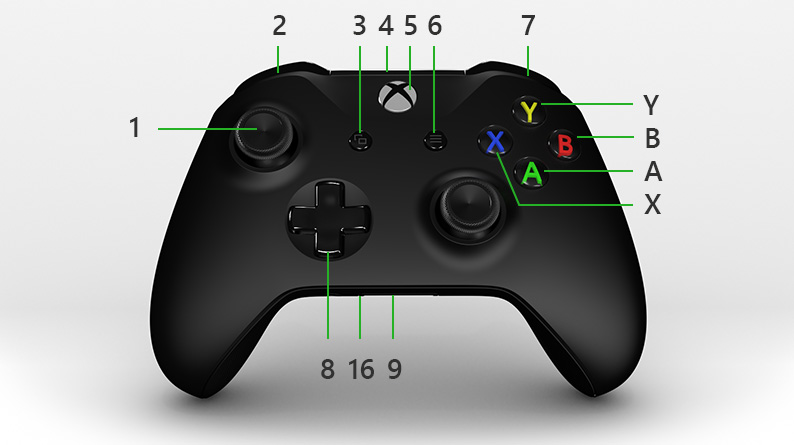
\includegraphics[scale=0.5]{images/vorderseite.jpg}
    \caption{Vorderseite des Controllers \cite{XboxController}(letzter Zugriff: 24.01.2025)}
    \label{fig:vorderseite}
\end{figure}

\begin{figure}[H]
    \centering
    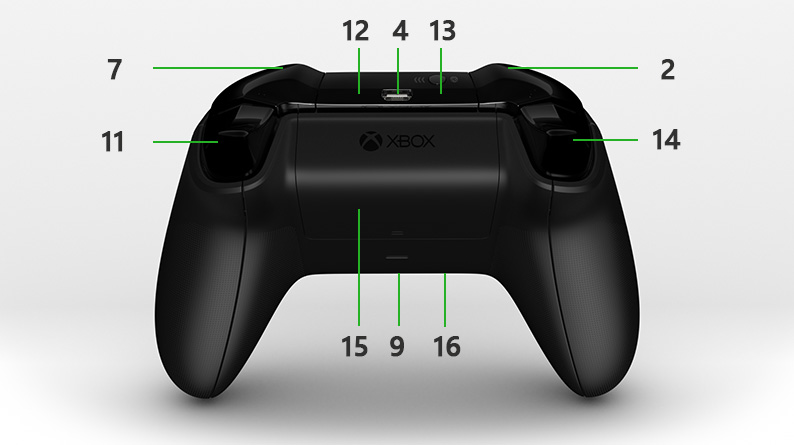
\includegraphics[scale=0.5]{images/rueckseite.jpg}
    \caption{Rückseite des Controllers \cite{XboxController}(letzter Zugriff: 24.01.2025)}
    \label{fig:rueckseite}
\end{figure}

\begin{table}[H]
    \begin{tabular}{|c|c|}
    \hline
    \rowcolor[gray]{0.8}
     Nummerierung der Taste & Funktion \\ \hline 
     1 & Bewegung des Ruders \\ \hline 
     2 & Reduzierung der linken Gashebelposition \\ \hline 
     7 & Reduzierung der rechten Gashebelposition \\ \hline
     11 & Erhöhung der rechten Gashebelposition \\ \hline
     14 & Erhöhung der linken Gashebelposition \\ \hline
     B + 2 & Umschalten des Rückwärtsgangs am linken Motor \\ \hline
     B + 7 & Umschalten des Rückwärtsgangs am rechten Motor \\ \hline
     B + 2 + 7 & Umschalten des Rückwärtsgangs an beiden Motoren \\
      & (basierend auf dem derzeitigen Gang am rechten Motor) \\ \hline
    \end{tabular}
\end{table}
Das Einlegen des Rückwärtsgangs ist durch eine Tastenkombination so gewählt, dass es nicht aus Versehen passieren kann.
Mit jeweils der Taste 2 oder 7 wird die Gashebelposition reduziert. Mit der zusätzlichen Betätigung der Taste B wird der 
Rückwärtsgang eingelegt an dem jeweiligen Motor. Wenn die Tasten 2, 7 und B gleichzeitig betätigt werden, 
wird der Rückwärtsgang für beide Motoren gleichzeitig umgeschalten. Dies ist so gewählt, da eine Verzögerung bei dem
Umschalten eines Rückwärtsgangs von 10 Sekunden eingebaut ist. Das soll dem Getriebe ermöglichen, den Gang zu wechseln
ohne eine direkte Gaseingabe. Nun muss es aber auch möglich sein, beide Rückwärtsgänge gleichzeitig umzuschalten, daher 
die vergleichsweise komplexe Tastenkombination.



\section{Integration des Rogue Device}
Damit der Controller die Steuerbefehle an das Schiff senden kann, muss das Rogue Device in das System integriert werden.
In diesem Fall ist das Rogue Device der Raspberry Pi. Damit dieser möglichst unbemerkt in das System integriert werden könnte,
muss der Controller drahtlos verbunden werden. Um eine unentdeckte Integration zu ermöglichen, muss die Art der Stromversorgung
unabhängig von dem Schiff sein. Dafür könnte ein Akku genutzt werden. Je nach Art der Anwendung kann der Akku 
Um die Kommunikation von dem Rogue Device zu dem Schiff zu ermöglichen, müssen
die einzelnen Systeme angesteuert werden. Um die Gashebelposition zu verändern, wird der Raspberry Pi mit dem Can-Bus des Schiffes
verbunden. \\
Die grobe Struktur des Rogue Devices soll wie folgt aussehen:
\begin{figure}[H]
    \centering
    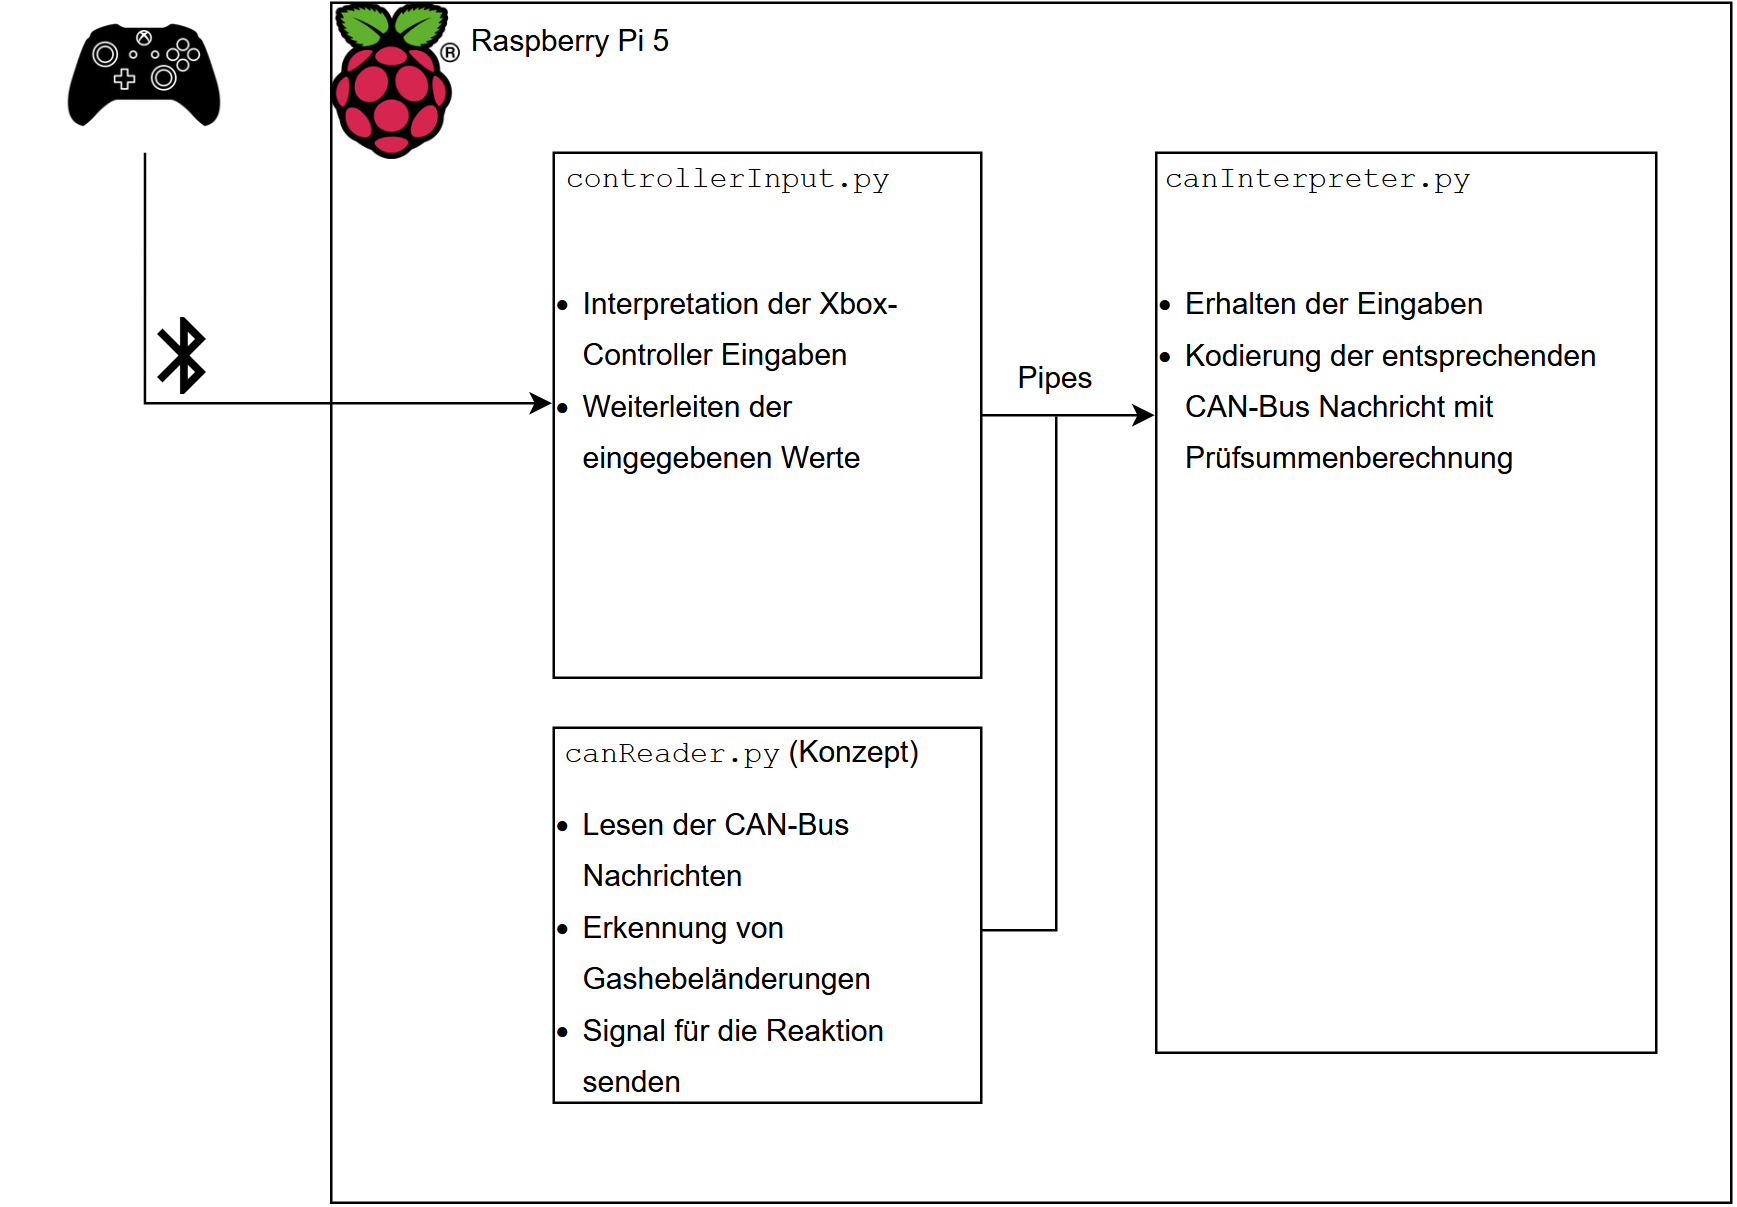
\includegraphics[scale=0.4]{images/piKonzept.png}
    \caption{Konzept der Programmstruktur auf dem Rogue Device}
    \label{fig:structureRogueDevice}
\end{figure}
Hier wird der Controller über Bluetooth mit dem Raspberry Pi verbunden. Dieser liest die Eingaben des Controllers aus und
sendet die entsprechenden Steuerbefehle an das Schiff. Dafür wird der Can-Bus des Schiffes genutzt. 
Sollte der Gashebel in der normalen Benutzung vom Schiffsführer benutzt werden, wird ein Signal an den Can-Bus gesendet. 
Dieses Signal wird dann an die Motoren weitergeleitet. Dafür wird \texttt{canReader.py} genutzt. Dieses Programm liest die
Nachrichten des Can-Bus reagiert auf die wichtigen Nachrichten für diese Arbeit.
Um diese Eingabe zu verhindern, muss auf diese Nachricht geachtet und reagiert werden. Mit dem Lesen des Can-Bus kann die 
entsprechende Nachricht entdeckt werden. Dann kann eine Nachricht von dem Rogue Device gesendet werden, um die Gashebelposition
zu überschreiben. Eigene Nachrichten müssen dazu erkannt werden, um eine Endlosschleife von eigenen Nachrichten zu verhindern. Dafür könnte
der Nachrichtenzähler überwacht werden. Aus den aufgezeichneten Nachrichten hat sich herausgestellt, dass der 
Nachrichtenzähler wenige verschiedene Werte hat. Daher sind diese Werte zu den eigenen erstellten Nachrichten 
verschieden. Dies ist eine einfache Methode, um die eigenen Nachrichten zu erkennen. Eine weitere Möglichkeit wäre,
eine eigene CAN-ID zu berechnen. Diese könnte dann genutzt werden, um die eigenen Nachrichten zu erkennen.
\\
konzept der Autopilot-Steuerung
\begin{itemize}
    \item Autopilot kommuniziert seriell mit Rudersteuerung
    \item Autopilot kann nur das Ruder steuern
    \item Autopilot-Nachrichten abfangen und analysieren
    \item evtl replayen in eigener Reihenfolge
    \item evtl eigene Nachrichten nachbauen
\end{itemize}


Wie in der Abbildung \ref{fig:j1939header} zu sehen, besteht der Header aus einer PGN, einer Quelladresse und einer Priorität. Um nun Nachrichten
an den Motor zu senden, kann eine Nachricht des Gashebels abgefangen werden. Die PGN kann für die eigene Nachricht genutzt
werden. Die Quelladresse kann man auch kopieren. Die Priorität sollte möglichst klein gewählt werden, 
damit die eigene Nachricht bevorzugt wird. In der eigenen Nachricht kann dann die gewünschte Gashebelposition gesendet werden.

\subsection{Rückmeldung der Eingaben}
Was muss ich dabei beachten?
Muss eine Rückmeldung für die Eingaben geschehen? Wenn ja, wie?
(kleiner OLED-Bildschirm oder App)
Es muss eine Art der Rückmeldung geben, um in etwa die Eingaben im Vergleich zum momentanen Zustand zu sehen.
Dabei sollte die Rückmeldung möglichst unauffällig sein. Ein kleiner OLED-Bildschirm könnte benutzt werden, allerdings
muss dieser physisch an den Raspberry Pi angeschlossen werden. Das würde die Versteckung des Rogue Devices erschweren.
Eine App auf einem Handy könnte die Rückmeldung geben. Diese App könnte dann die gewünschten Positionen anzeigen.
Dafür muss der Raspberry Pi mit dem Handy verbunden werden. Dies könnte über Bluetooth geschehen.
Hier ist zu beachten, dass die Verbindung stabil ist und nicht von anderen Geräten gestört wird.
Jedoch kann ist hier mit einem größeren Aufwand zu rechnen, da die App erst entwickelt werden muss.
Eine weitere Möglichkeit würden Vibrationen im Xbox Controller sein. Diese könnten genutzt werden, wenn die derzeitige
Eingabe ein Maximum oder Minimum erreicht hat. Allerdings ist dies nicht so genau wie eine Anzeige auf einem Bildschirm.
Es könnten auch nur wenige bestimmte Positionen mittgeteilt werden. \\
Eine solche Rückmeldung ist wichtig, um eine sogenannte Pilot Induced Oscillation (PIO) zu verhindern. Das Phänomen tritt
vorallem bei Flugzeugen auf, wenn der Pilot zu stark gegensteuert. Dabei reagiert das Flugzeug auf die Steuerbefehle
des Piloten und der Pilot reagiert auf die Reaktion des Flugzeugs. Dies führt zu einer Schwingung, die sich immer weiter
verstärkt. \cite{McRuer1995} \\
Ein vergleichbares Phänomen kann auch bei Schiffen auftreten, wenn auch nicht im gleichen Ausmaß. Bei Schiffen 
sind die Bewegungen im Wasser langsamer und weniger stark. Dennoch kann es zu einer Schwingung kommen, wenn der Schiffsführer
zu stark gegensteuert. Um dies zu verhindern, ist eine Rückmeldung der Eingaben wichtig. Diese Rückmeldung kann dann
dazu genutzt werden, um die Eingaben genauer zu wählen.